\documentclass{elegantpaper}

\title{分布式空间top-k频繁关键字查询}

\author{
    冯运 1160300524 %
    \\[0.5ex] %
    陈进龙 1160300525 %
}

\begin{document}

\maketitle

\begin{abstract}
\end{abstract}

\section{问题描述}

随着社交软件的大量出现,许多社交平台允许用户在发布消息的时候会标记他们的地理位置,例如微博,微信朋友圈等.这样的背景条件下,就产生了新的数据分析问题.例如,当用户想去知道附近的热门地点时,需要对已经产生的地点信息进行计算,即用户给定一片空间区域,然后查询返回k个最热门的关键词,而随着数据产生的越来越多,数据量的存储已经远远超过了一个单机的能力,所以分布式的空间top-k关键字查询就成为了新的数据分析需求.

\subsection{形式化描述}
我们使用$L=\{o_1,o_2,o_3,...,o_n\} $ 来表示一个包含N个o对象的数据集,每一个对象$o_i$是<Place,Words>形式的对象.Place是一个n维的的空间坐标点,用$Place=\{w_1,w_2,...\}$来表示,而Words是对象o保存的关键字,用$Words=\{w_1,w_2,w_3... \}$.\newline
使用$V=\{U_{o\in L}O.Words\}$来表示L内的所有关键词的集合,使用$f_o(w)$来表示关键词$w$出现在对象o中的次数.\newline
对于一个给定的查询区域R,则可以用$f_R(w)=\{\sum{f_{oi(w)|o_i.Place\in R}} \}$来表示关键词w在区域R中出现的频率(次数).\newline
对于这个top-k频繁关键词查询系统来说,输入一个查询条件:$<R_Q,k>$,$R_Q$指明了选择的查询区域,k指明了最终输出的k个关键字,而这k个关键字是出现在$R_Q$区域内的k个最高频的关键字.\newline

\subsection{举例}

例如figure1表示的是一个二维的平面,其中包含了8个对象,则可以用$L=\{o_1,o_2,o_3,o_4,o_5,o_6,o_7,o_8\}$,每一个对象对应的关键词组在table1中展示
假设用户的查询是$Query=<R_4,3>$,即查询的区域是R4,用户要求的k=3的情况下,需要返回在区域R4中的top-3频繁的关键字,而从figure1中可以看出,在R4中包含的对象有$\{o_4,o_6,o_7,o_8\}$,根据table1可以算出最终的top-3为$\{w_2,w_3,w_9\}$.

\begin{figure}[!ht]
	\centering
	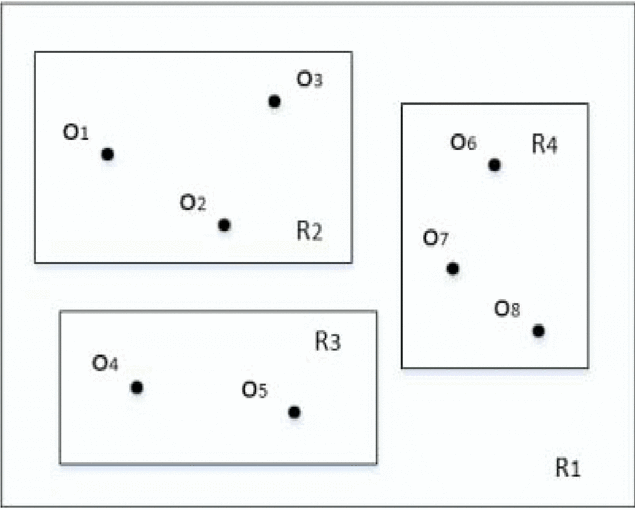
\includegraphics[width=0.6\textwidth]{figure1.png}
	\caption{空间示意图\label{fig:figure1}}
\end{figure}

\begin{table}[!htbp]
    \small
    \centering
    \caption{对象的关键词}
      \begin{tabular}{cccc}
      对象&关键词&对象&关键词\\
      \hline
      $o_1$   & $\{w_2,w_3,w_5\}$ & $o_5$&$\{w_1,w_1,w_3,w_5\}$\\
      $o_2$   & $\{w_1,w_4,w_5\}$ & $o_6$&$\{w_4,w_7,w_9\}$\\
      $o_3$   & $\{w_2,w_4,w_4\}$ & $o_7$&$\{w_2,w_2,w_3,w_5\}$\\
      $o_4$   & $\{w_3,w_8,w_9,w_9\}$ & $o_8$&$\{w_3,w_3,w_6\}$\\
      \end{tabular}
\end{table}

\section{系统设计}

本节首先介绍一种分布式的索引结构,并基于此结构实现一种简单的查询算法。然后介绍基于此设计的一些改进以及相应的新的查询算法。

\subsection{索引结构}

对于空间数据索引,首选的结构就是R树。
但是传统的R树是基于单机的,没有考虑分布式计算的需求,这里我们介绍一种分布式的R树 [1] ,可以满足并行计算的要求。

\subsubsection{MC-R树}

MC-R树是一种分布式的多维数据索引结构,它将物理计算节点分为两类:

\begin{itemize}

    \item Master节点:保存全局索引信息。Master维护着一个\verb|<MBR, client_id>|的列表以及在其上的R树索引,用于将查询转发到相应的Client节点;
    
    \item Client节点:负责保存局部索引以及数据。Client节点保存实际的数据分块以及在这些数据上建立的局部R树索引;
    
\end{itemize}

\begin{figure}[!ht]
    \centering
    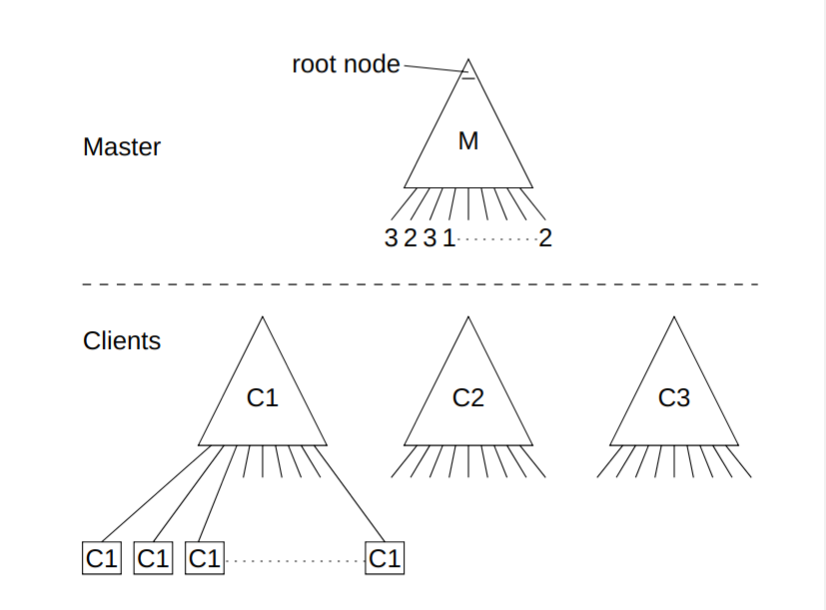
\includegraphics[width=0.6\textwidth]{figure/MC-Rtree.png}
    \caption{MC-R树的结构,其中三角形表示物理节点,四边形表示数据}
\end{figure}

\noindent MC-R树的建立过程如下:

\begin{itemize}
    
    \item[1.] 数据划分:Master节点将导入的按照特定的划分算法数据划分为G组,每一组最多M个数据。其中M是每一个物理节点能保存的最大数据量;
    
    \item[2.] 数据分配:数据划分完成后,将每一组数据分配给一个Client节点,并将该次分配产生的\verb|<MBR, client_id>|二元组添加到列表中;
  
    \item[3.] 建立全局索引:Master将数据分配到Client节点后,在分配过程中产生的\verb|<MBR, client_id>|列表上建立R树索引;
    
    \item[4.] 建立局部索引:收到数据的Client节点将数据保存到本地磁盘,然后在这些数据上建立局部R树索引。
 
\end{itemize}

\noindent 对于数据的划分,这里给出两种比较典型的多维数据划分算法:

\begin{itemize}
    
    \item Hilbert packing算法:将所有的数据(超立方体)按照它们的中心到希尔伯特曲线起点的距离进行排序,然后将排序结果等距离的划分为G段即可。
    
    \item Sort-Tile-Recursive(STR)算法:对于n个k维的数据(超立方体),首先确定需要划分成的份数$G = \lceil \frac{n}{M} \rceil$。接下来将这些超立方体按照它们中心的第一维坐标进行排序,将排序结果等距离地分为$S = \lceil G^{\frac{1}{k}} \rceil$份,然后递归的对每一份的$k - 1$维坐标进行处理,最终得到划分结果。

\end{itemize}

\subsection{执行查询}



\section{工作流程}
\subsection{请求过程}
\begin{itemize}
    \item[1.] 用户向查询集群发送查询请求$<R_Q,k>$
    \item[2.] 集群将此次请求的处理任务分配到查询集群的某个计算结点$N_i$上
    \item[3.] 结点$N_i$收到这个查询请求后,为这个请求编号为$Q_j$,为这个请求做相应的初始化工作,包括分配一个大小为K的大根堆,分配一个查询结点队列QueryQueue(用于保存需要$N_i$需要查询的索引结点),这个队列中初始时只有索引R树的根节点
    \item[4.] 向QueryQueue中的所有索引结点发送查询请求,然后在收到所有查询结点相应的响应后,将所有查询结点弹出QueryQueue,然后将响应中包含的新的查询结点加入QueryQueue
    \item[5.] 重复步骤4,直到最终队列中只有索引树的叶结点时,直接向所有的索引树叶结点发送查询请求,之后保留QueryQueue不变
\end{itemize}
\subsection{索引过程}
\begin{itemize}
    \item[1.] 对应于请求过程中的步骤4,在一个索引树的非叶子结点收到结点$N_i$的查询请求后,根据请求中的查询区域$R_Q$,检索自己的已有的索引,然后得到下一级索引记录所在的子索引树结点,将这些结点返回给结点$N_i$.
    \item[2.] 对应于请求过程的步骤5,在一个索引树的叶子节点收到结点$N_i$的查询请求后,根据请求中的查询区域$R_Q$,找到所有存储在自己结点的所有包含在区域$R_Q$中的记录\verb|<t, t.entries, t.freq>|,然后根据关键词t将具有相同关键词t的记录全部发向同一个计算结点$C_k$
\end{itemize}
\subsection{计算过程}
\begin{itemize}
    \item[1.] 对应于索引过程的步骤2,在收到来自索引树的叶子结点的所有记录后,根据\verb|<t, t.entries, t.freq>|将具有相同的关键词t的记录聚集在一起,将其出现频率\verb|t.freq|累加在一起
    \item[2.] 
\end{itemize}
\end{document}